{{ % Localize command definitions

\newcommand{\Rationals}{\mathbb{Q}}
\newcommand{\Booleans}{\mathbb{B}}

\chapter{Class 7}

For this chapter, we replace the word \emph{formula} in rules and 
proofs of a formal system by the word \emph{judgement}.

\section{Natural Deduction for Propositional Logic}

Judgements in Natural Deduction have the form $\Gamma \vdash \phi$, 
where $\Gamma$ is a set of formulas and $\phi$ is a formula.
Semantically, for all interpretations $v$, if all formulas in 
$\Gamma$ are true in $v$, then $\phi$ is true in $v$.
Formal system for natural deduction defines a meta-symbol 
$\vdash_\text{meta}$ such that  $\vdash_\text{meta} (\Gamma \vdash 
\phi)$. 

\subsection{Judgements in Natural Deduction}

We use the notation $\Gamma, \phi$ to show $\Gamma \cup \{\phi\}$. 

\begin{enumerate}
  \item Axioms
  \[ \infer* [right=ax]
    { }{\Gamma, \phi \vdash \phi}
    \qquad\qquad \infer* [right=$\top$-intro]
    { }{\Gamma \vdash \top}
  \]
  
  \item False-elimination: if $\bot$ can be derived, then anything 
  can be derived.
  \[ \infer* [right=$\bot$-elim]
    {\Gamma \vdash \bot}{\Gamma \vdash \phi}
  \]

  \item Conjunction elimination and introduction
  \[ \infer* [right=$\land$-elim]
    {\Gamma \vdash \phi \land \psi}{\Gamma \vdash \phi}
    \qquad\qquad \infer* [right=$\land$-elim]
    {\Gamma \vdash \phi \land \psi}{\Gamma \vdash \psi}
    \qquad\qquad \infer* [right=$\land$-intro]
    {\Gamma \vdash \phi \\ \Gamma \vdash \psi}
    {\Gamma \vdash \phi \land \psi}
  \]

  \item Disjunction elimination and introduction
  \[ \infer* [right=$\lor$-elim]
    {\Gamma \vdash \phi \lor \psi 
    \\ \Gamma, \phi \vdash \chi
    \\ \Gamma, \psi \vdash \chi}{\Gamma \vdash \chi}
    \qquad\qquad \infer* [right=$\lor$-intro]
    {\Gamma \vdash \phi}{\Gamma \vdash \phi \land \psi}
    \qquad \infer* [right=$\land$-intro]
    {\Gamma \vdash \phi}{\Gamma \vdash \psi \land \phi}
  \]

  \item Negation elimination and introduction
  \[ \infer* [right=$\neg$-elim]
    {\Gamma \vdash \phi \\ \Gamma \vdash \neg \phi}
    {\Gamma \vdash \bot}
    \qquad\qquad \infer* [right=$\neg$-intro]
    {\Gamma, \phi \vdash \bot}{\Gamma \vdash \neg \phi}
  \]
  \item Implication elimination and introduction
  \[ \infer* [right=$\rightarrow$-elim]
    {\Gamma \vdash \phi \\ \Gamma \vdash \phi \rightarrow \psi}
    {\Gamma \vdash \psi}
    \qquad\qquad \infer* [right=$\rightarrow$-intro]
    {\Gamma, \phi \vdash \psi}{\Gamma \vdash \phi \rightarrow \psi}
  \]
  Observe how $\rightarrow$-elim is similar to modus ponens.
\end{enumerate}

\begin{homework}
  Prove implication transitivity using Natural Deduction.
\end{homework}

\begin{example}\label{lecture_7:contrapositive}
  Show $(\phi \rightarrow \psi) \rightarrow 
  (\neg \psi \rightarrow \neg \phi)$.
\end{example}
\begin{proof}
  \[ \infer* [right=$\rightarrow$-intro]
    { \infer* [right=$\rightarrow$-intro]
      { \infer* [right=$\neg$-intro]
        { \infer* [right=$\neg$-elim]
          { \phi \rightarrow \psi, \neg \psi, \phi \vdash \psi \\
            \phi \rightarrow \psi, \neg \psi, \phi \vdash \neg \psi
          }{\phi \rightarrow \psi, \neg \psi, \phi \vdash \bot}
        }{\phi \rightarrow \psi, \neg \psi \vdash \neg \phi}
      }{(\phi \rightarrow \psi) 
        \vdash (\neg \psi \rightarrow \neg \phi)}
    }{\vdash (\phi \rightarrow \psi) 
      \rightarrow (\neg \psi \rightarrow \neg \phi)}
  \]
  Now we have two goals to prove. 
  \[ \infer* [right=$\rightarrow$-elim]
    { \infer* [right=ax]
      { }{\phi \rightarrow \psi, \neg \psi, \phi \vdash \phi} \\
      \infer* [right=ax]
      { }{\phi \rightarrow \psi, \neg \psi, \phi 
          \vdash \phi \rightarrow \psi}
    }{\phi \rightarrow \psi, \neg \psi, \phi \vdash \psi}
    \qquad \infer* [right=ax]
      { }{\phi \rightarrow \psi, \neg \psi, \phi \vdash \neg \psi}
    \qquad 
  \]
\end{proof}

Observe how this method of writing proofs in Natural Deduction
requires us to rewrite the context for every step. We can use a
slightly different notation to avoid this repetition.

We can draw boxes to introduce \emph{contexts} in a proof. Every
formula written inside a box is assumed to hold only within that box.
The following ``proofs'' are examples of using this notation.

\[ \infer {
  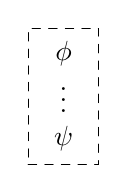
\begin{tikzpicture}
    \node [draw, rectangle, dashed, line cap=round]
    {\begin{tabular}{c} $\phi$ \\ \vdots \\ $\psi$ \end{tabular}};
  \end{tikzpicture}
  }{\phi \rightarrow \psi}
  \qquad \infer {
  \begin{tikzpicture}
    \node [draw, rectangle, dashed, line cap=round]
    {\begin{tabular}{c} $\phi$ \\ \vdots \\ $\bot$ \end{tabular}};
  \end{tikzpicture}
  }{\neg \phi}
  \qquad \infer {
  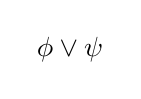
\begin{tikzpicture}
    \node {$\phi \lor \psi$};
  \end{tikzpicture} \\
  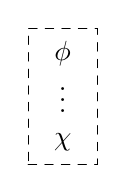
\begin{tikzpicture}
    \node [draw, rectangle, dashed, line cap=round]
    {\begin{tabular}{c} $\phi$ \\ \vdots \\ $\chi$ \end{tabular}};
  \end{tikzpicture} \\
  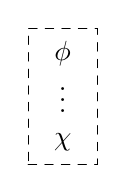
\begin{tikzpicture}
    \node [draw, rectangle, dashed, line cap=round]
    {\begin{tabular}{c} $\phi$ \\ \vdots \\ $\chi$ \end{tabular}};
  \end{tikzpicture}
  }{\chi}
\]

Using this notation, we can rewrite the proof for example
\ref{lecture_7:contrapositive}:
\[ \infer {
  \begin{tikzpicture}
    \node [draw, rectangle, dashed, line cap=round] {$
    \infer {
      \text{1. } \phi \rightarrow \psi \\\\
      \begin{tikzpicture}
        \node [draw, rectangle, dashed, line cap=round] {$
        \infer {
          \text{2. } \neg \psi \\\\
          \begin{tikzpicture}
            \node [draw, rectangle, dashed, line cap=round] {
            \begin{tabular}{c}
              3. $\phi$ \\
              4. $\psi$ ($\rightarrow$-elim, 1, 3) \\
              5. $\bot$ ($\neg$-elim, 2, 4)
            \end{tabular}
            };
          \end{tikzpicture}
        }{\neg \phi}
        $};
      \end{tikzpicture}
    }{\neg \psi \rightarrow \neg \phi}
    $};
  \end{tikzpicture}
  }{(\phi \rightarrow \psi)
    \rightarrow (\neg \psi \rightarrow \neg \phi)}
\]

The system defined above is in fact the NJ (Intuitionistic Natural 
Deduction) system. The following rule, namely the law of excluded
middle, cannot be derived in NJ:
\[ \infer* [right=ex-middle]
  { }{\Gamma \vdash \phi \lor \neg \phi}
\]

The NK system (Classical Natural Deduction) is NJ with the addition
of the law of excluded middle. The NK system is sound and complete
for propositional logic.

Assumption of the law of excluded middle is in fact an important
distinction between Intuitionistic and classical logic. In the
following is an example which uses excluded middle in its proof.

\begin{example}
  Show that there exist $a, b \not \in \Rationals$ such that
  $a ^ b \in \Rationals$.
\end{example}
\begin{proof}
  Let $a = \sqrt{2} ^ {\sqrt{2}}$ and $b = \sqrt{2}$. We know that
  $\sqrt{2} \not \in \Rationals$. We do a ``classical''
  case-splitting on $a \in \Rationals$:
  \begin{enumerate}
    \item $a \not \in \Rationals$. We have
    \[ a ^ b
      = \left( \sqrt{2} ^ {\sqrt{2}} \right) ^ {\sqrt{2}}
      = \sqrt{2} ^ 2
      = 2 \in \Rationals \]
  \item $a \in \Rationals$. We are already done with the proof; let
  $a_1 = b_1 = \sqrt{2}$. We know $a_1, b_1 \not \in \Rationals$ and,
  by assumption, ${a_1} ^ {b_1} \in \Rationals$.
  \end{enumerate}

  Observe how this classical-style proof utilizes the law of excluded
  middle in the case-splitting: $\sqrt{2} ^ {\sqrt{2}}$ is either in
  $\Rationals$ or not in $\Rationals$; there is no \emph{middle}.
\end{proof}

\section{Kripke Semantics}

Classically, an interpretation $v: P \to \Booleans$ is defined as a
mapping from a set of propositions to boolean values $\top$ and
$\bot$. For intuitionistic reasoning, we define a new semantics.

\begin{definition}
  A Kripke model $m$ is defined as a tuple $(W, \leq, w_0,
  v: W \times P \to \Booleans)$, where $W$ is a set of classical
  worlds, $\leq$ is a pre-order relation on $W$, $w_0$ is the initial
  world, and $v$ is a function from pairs of world and proposition
  to boolean values such that for any $w, w' \in W$ and any
  $p \in P$, if $w \leq w'$, then $v(w, p) \leq v(w', p)$.
\end{definition}

Informally, a Kripke model is an interpretation model for
intuitionistic proof systems. The following facts hold for any Kripke
model $m$:
\begin{enumerate}
  \item $m \models \phi$ iff $m \vdash_{w_0} \phi$.
  \item $m \not \models_w \bot$ for any world $w$.
  \item $m \models_w p$ iff $v(w, p) = \top$.
  \item $m \models_w \phi \rightarrow \psi$ iff for any $w'$, if
  $w \leq w'$ and $m \models_{w'} \phi$, then $m \models_{w'} \psi$.
\end{enumerate}

In NJ, whenever you show $\phi \lor \psi$, you need to show either
$\phi$, or $\psi$. As previously stated, the law of excluded middle
cannot be derived in NJ. To show this, we need to show that there
exists a Kripke model $m$ such that excluded middle is false in a
world $w$ of $m$.

Let us define a Kripke model with only one proposition $p$ and only
two worlds $w_0$ and $w_1$, where $w_0 \leq w_1$, and $p$ is false in
$w_0$ and true in $w_1$.

\begin{center}
  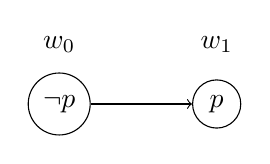
\begin{tikzpicture}
    \node (w0) at (0, 0) [draw, circle] {$\neg p$};
    \node (w1) at (2, 0) [draw, circle] {$p$};
    \node at (0, .75) {$w_0$};
    \node at (2, .75) {$w_1$};
    \draw[->] (w0) -- (w1);
  \end{tikzpicture}
\end{center}

Let us examine what formulas are true (or false) in each world. By
definition, $p$ is false in $w_0$. Let us examine the value of
$\neg p$ in $w_0$. We can safely substitute $\neg p$ with $p
\rightarrow \bot$. By definition, $p \rightarrow \bot$ holds in
$w_0$ iff for any world $w$, if $w_0 \leq w$ and $p$ is true in $w$,
then $\bot$ is true in $w$. We know $p$ is true in $w_1$. We also
know that $\bot$ is not true in $w_1$, as it is not true in any world.
So, by definition, $p \rightarrow \bot$ is false in $w_0$. So, both
$p$ and $\neg p$ are false in $w_0$, from which we obtain that $p
\lor \neg p$ is also false in $w_0$.

\section{Sequent (Gentzen) Calculus and LK}

Judgements in the LK proof system have the form $\Gamma \vdash
\Delta$, where both $\Gamma$ and $\Delta$ are sets of formulas.
Judgement $\Gamma \vdash \Delta$ should be read as ``the
\emph{conjunction} of the formulas in $\Gamma$ implies the
\emph{disjunction} of the formulas in $\Delta$''. Semantically, for
a classical interpretation $v$, $v \models (\Gamma \vdash \Delta)$
if and only if, if all formulas in $\Gamma$ are true under $v$, then
some fomula in $\Delta$ is true under $v$.

\subsection{Judgements in LK}

Observe how every non-axiom judgement increases the number of logical
connectives in the set of formulas.

\begin{enumerate}
  \item Axioms
  \[ \infer* [right=ax]
    { }{\Gamma, \phi \vdash \phi, \Delta}
    \qquad\qquad \infer* [right=$\bot$-elim]
    { }{\Gamma, \bot \vdash \Delta}
    \qquad\qquad \infer* [right=$\top$-intro]
    { }{\Gamma \vdash \top, \Delta}
  \]
  \item Conjunction
  \[ \infer
    {\Gamma, \phi, \psi \vdash \Delta}
    {\Gamma, \phi \land \psi \vdash \Delta}
    \qquad\qquad \infer
    {\Gamma \vdash \phi, \Delta
    \\ \Gamma \vdash \psi, \Delta}
    {\Gamma \vdash \phi \land \psi, \Delta}
  \]
  \item Disjunction
  \[ \infer
    {\Gamma, \phi \vdash \Delta
    \\ \Gamma, \psi \vdash \Delta}
    {\Gamma, \phi \lor \psi \vdash \Delta}
    \qquad\qquad \infer
    {\Gamma \vdash \phi, \psi, \Delta}
    {\Gamma \vdash \phi \lor \psi, \Delta}
  \]
  \item Negation
  \[ \infer
    {\Gamma, \phi \vdash \Delta}
    {\Gamma \vdash \neg \phi, \Delta}
    \qquad\qquad \infer
    {\Gamma \vdash \phi, \Delta}
    {\Gamma, \neg \phi \vdash \Delta}
  \]
  \item Implication
  \[ \infer
    {\Gamma, \phi \vdash \psi, \Delta}
    {\Gamma \vdash \phi \rightarrow \psi, \Delta}
    \qquad\qquad \infer
    {\Gamma \vdash \phi, \Delta
    \\ \Gamma, \psi \vdash \Delta}
    {\Gamma, \phi \rightarrow \psi \vdash \Delta}
  \]
\end{enumerate}

The LK proof system is sound and complete for propositional logic.
This actually means that excluded middle can be derived in LK.

\begin{homework}
  Prove the following in LK:
  \begin{enumerate}
    \item The law of excluded middle: $ \vdash p \lor \neg p$,
    \item Implication transitivity.
  \end{enumerate}
\end{homework}

}} % End localization of command definitions
